\section{Gaussian Splatting Renderer}
\label{sec:renderer}

\subsection{Mathematical Formulation}

Each Gaussian $k$ is characterised by a covariance matrix

\begin{equation}
  \Sigma_k =
  \begin{pmatrix}
    \sigma_{x,k}^2 & \rho_k\,\sigma_{x,k}\sigma_{y,k} \\
    \rho_k\,\sigma_{x,k}\sigma_{y,k} & \sigma_{y,k}^2
  \end{pmatrix},
  \label{eq:covariance}
\end{equation}

\noindent which defines an unnormalised 2-D Gaussian kernel on a $[-5,5]^2$ grid:

\begin{equation}
  G_k(\mathbf{u}) = \exp\!\Bigl(-\tfrac{1}{2}\,\mathbf{u}^\top \Sigma_k^{-1} \mathbf{u}\Bigr),
  \quad \mathbf{u} \in [-5, 5]^2.
  \label{eq:kernel}
\end{equation}

The kernel is normalised to unit peak ($G_k \leftarrow G_k / \max G_k$),
padded to $H \times W$, then translated to position $(x_k, y_k)$ via an affine
transformation.  The final image is the additive composition:

\begin{equation}
  \hat{\I}_{ij} = \mathrm{clamp}\!\left(
    \sum_{k=1}^{K} c_k \cdot G_k^{(x_k,y_k)}(i,j),\; 0, 1
  \right),
  \label{eq:compositing}
\end{equation}

\noindent where $G_k^{(x_k,y_k)}$ denotes the translated kernel.

\subsection{Implementation Details}

The renderer is implemented in \texttt{src/utils/gaussian\_to\_image.py} using
PyTorch's \texttt{F.affine\_grid} and \texttt{F.grid\_sample} for the translation.
Important implementation notes:

\paragraph{Covariance inversion.}
We use \texttt{torch.linalg.inv} (replacing the deprecated \texttt{torch.inverse})
for numerically robust inversion.
If $\det(\Sigma_k) \leq 0$ (which can occur for extreme $\rho$ values), a small
$\epsilon = 10^{-6}$ is added to the diagonal to restore positive-definiteness.

\paragraph{Kernel maximum clamping.}
The normalisation divisor $\max_{\mathbf{u}} G_k(\mathbf{u})$ is clamped to
$\geq 10^{-8}$ to prevent division-by-zero on near-zero kernels.

\paragraph{Channel handling.}
The renderer supports $C$ channels (default $C=1$ for greyscale).
For MNIST we use $C=1$; the code extends to RGB without modification.

\subsection{Coordinate Convention}
\label{sec:coord_convention}

Understanding the coordinate convention of \texttt{F.affine\_grid} is critical.
The affine transformation is defined by a $2 \times 3$ matrix $\theta$:

\begin{equation}
  \theta =
  \begin{pmatrix}
    1 & 0 & t_x \\
    0 & 1 & t_y
  \end{pmatrix}.
  \label{eq:theta}
\end{equation}

\noindent PyTorch's \texttt{F.affine\_grid} with \texttt{align\_corners=True}
maps each \emph{output} pixel at normalised position $\mathbf{g}$ to an \emph{input}
sample position $\mathbf{s} = \mathbf{g} + \mathbf{t}$.
In other words, setting $t_x = c > 0$ means output pixel at $g_x = 0$ (centre)
samples the input at $s_x = c$, effectively \emph{shifting the content to the left}.

\medskip
\noindent
\textbf{Key consequence:} a Gaussian kernel centred at input $s_x = 0$ with
translation $t_x = c$ appears at \emph{output} position $g_x = -c$.
Equivalently, to render a Gaussian at output position $x_\text{render}$,
the translation parameter must satisfy $t_x = -x_\text{render}$,
so the coordinate stored in $\Wraw_{k,5}$ must be
\begin{equation}
  \Wraw_{k,5} = \atanh(-x_\text{pixel}),
  \label{eq:coord_fix}
\end{equation}
where $x_\text{pixel} \in [-1,1]$ is the desired normalised pixel position.
This convention is illustrated in Figure~\ref{fig:coord_inversion}.

\begin{figure}[htbp]
  \centering
  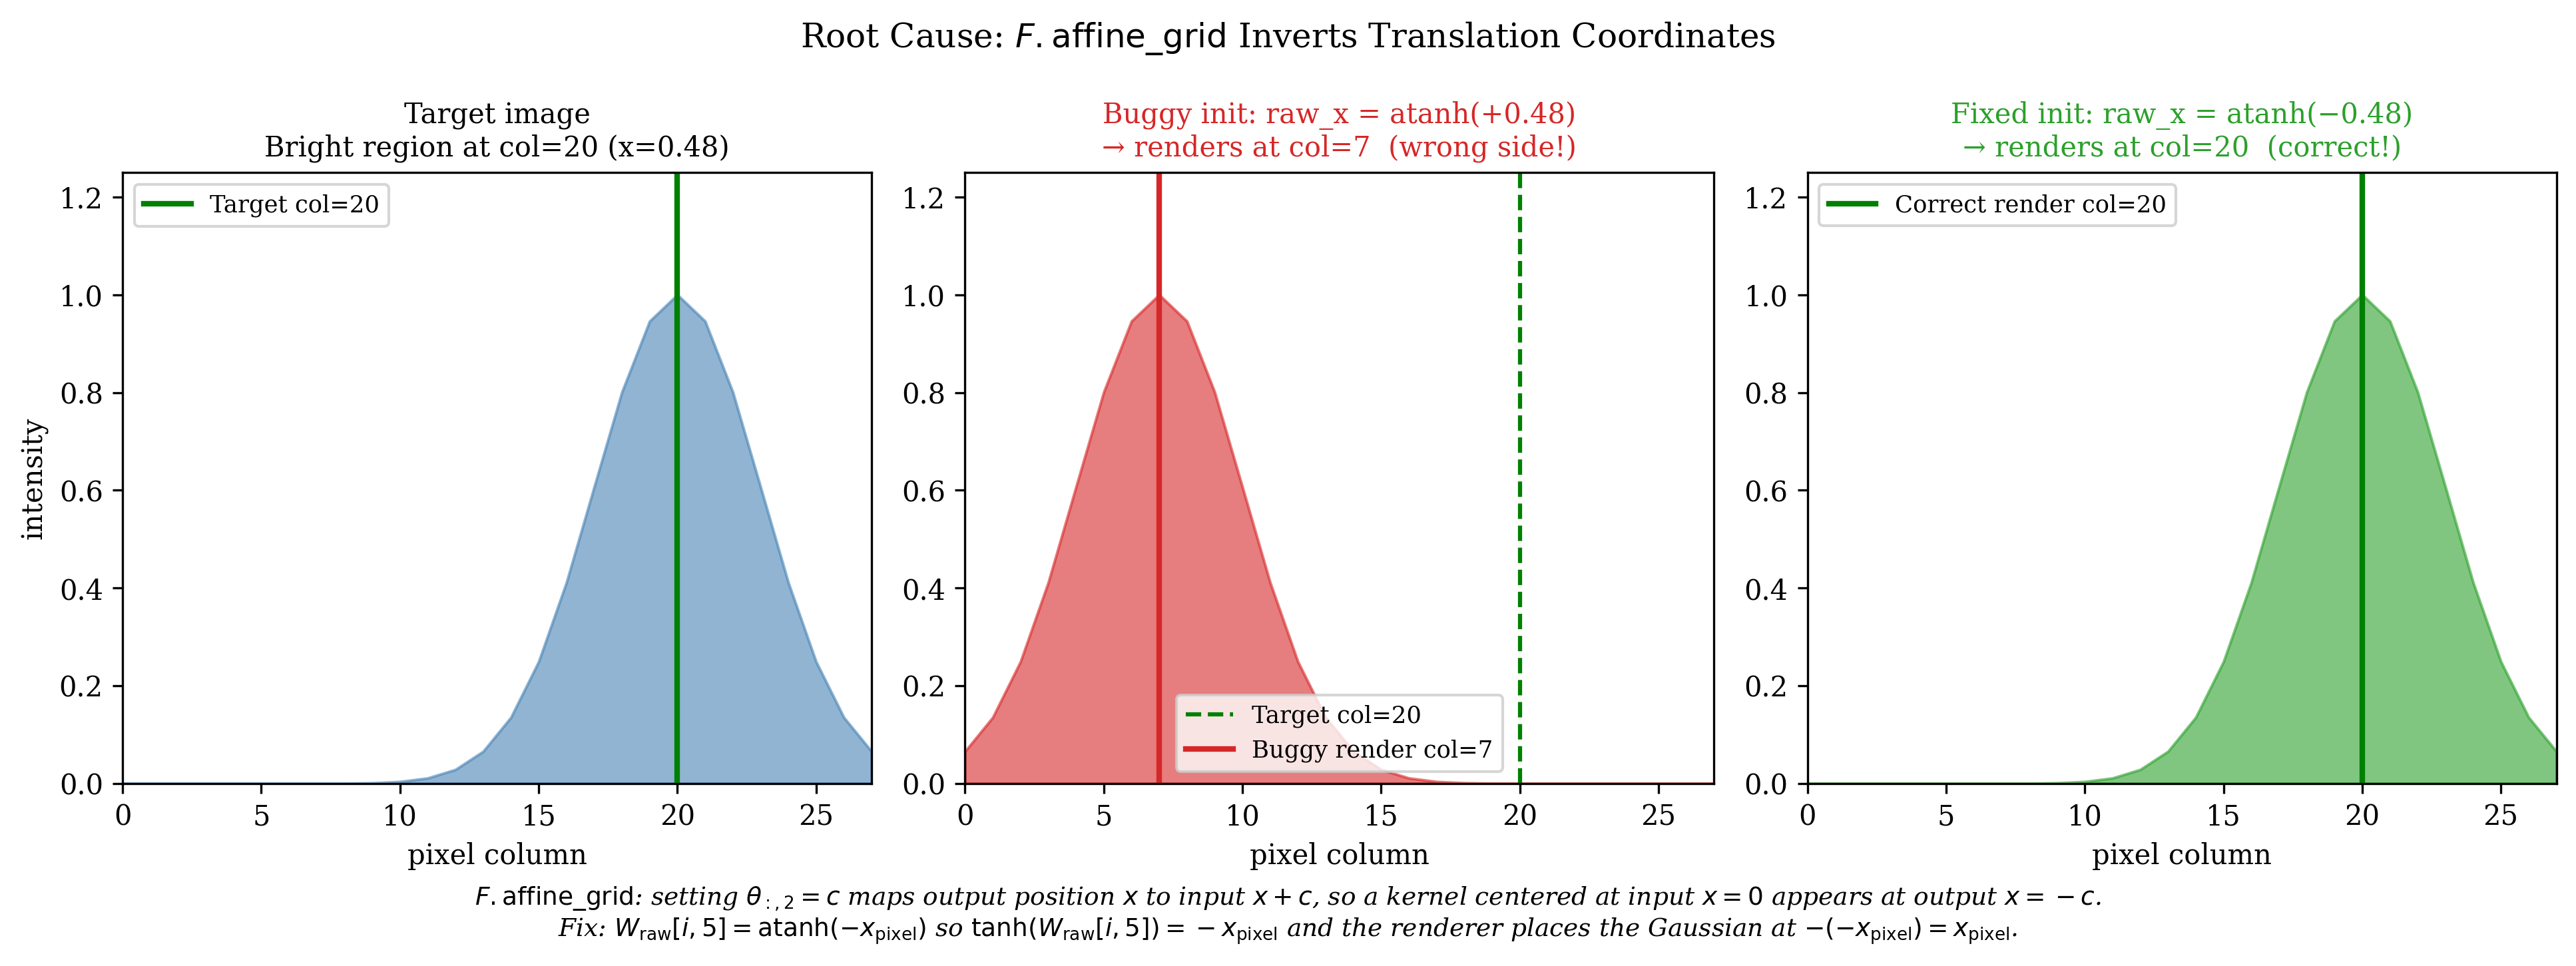
\includegraphics[width=\linewidth]{figures/fig_09_coord_inversion_diagram.png}
  \caption{%
    \textbf{Coordinate inversion in the renderer.}
    \emph{Left:} target image with a bright region at column~20 ($x \approx +0.48$).
    \emph{Centre:} with the buggy initialisation ($\Wraw_{k,5} = \atanh(+0.48)$),
    the Gaussian renders at column~$\approx 6$ (wrong side).
    \emph{Right:} with the corrected initialisation ($\Wraw_{k,5} = \atanh(-0.48)$),
    the Gaussian renders at column~20 (correct).
    The formula at the bottom summarises the \texttt{F.affine\_grid} convention.%
  }
  \label{fig:coord_inversion}
\end{figure}
